\section{联合熵与条件熵}
\label{sec:info-joint-conditional}

有两个变量$X,Y$时，可以问两种问题：把有序对$(X,Y)$一起确定，平均要多少信息；已经知道$Y$以后，确定$X$还需要多少信息。前者只要把$(X,Y)$看成一个随机对象，后者要用条件分布。本节先分别定义这两个量，再说明它们怎样由“先揭示一个、再揭示另一个”的分解连接起来。

\subsection{联合熵}
\label{sec:info-joint-entropy}

有序对$(X,Y)$本身是一个离散随机对象，取值于$\mathcal{X}\times\mathcal{Y}$，联合概率质量$p_{X,Y}(x,y)$构成一张概率表。熵只依赖概率表，所以可以直接套用式~\eqref{eq:info-entropy}。

\begin{definition}[联合熵]
\label{def:info-joint-entropy}
离散随机变量$X,Y$的\term{联合熵}（joint entropy）是
\begin{equation}
  H(X,Y)=-\sum_{x,y}p_{X,Y}(x,y)\ln p_{X,Y}(x,y)=\mathbb{E}[-\ln p_{X,Y}(X,Y)].
  \label{eq:info-joint-entropy}
\end{equation}
多个变量的联合熵$H(X_1,\dots,X_n)$同样定义。若$(X,Y)$有联合密度$f_{X,Y}$，在$f_{X,Y}\lvert\ln f_{X,Y}\rvert$可积时，联合微分熵$h(X,Y)$定义为$-\iint f_{X,Y}\ln f_{X,Y}\,\mathrm{d}x\,\mathrm{d}y$。
\end{definition}

联合熵并不由两个边缘分布决定。图~\ref{fig:info-same-marginals}的三张表，$X$与$Y$的边缘都是公平硬币，$H(X)=H(Y)=\ln2$。独立时四格各$\tfrac14$，联合熵是$\ln4\approx1.386$ nat，正好是$H(X)+H(Y)$。$Y=X$时只有对角线两格有质量，联合熵只有$\ln2$：知道$X$就知道$Y$，有序对并不比单个变量更难确定。第三张表是公平硬币经过以概率$\tfrac14$出错的线路，
\[
  H(X,Y)=-2\cdot\tfrac38\ln\tfrac38-2\cdot\tfrac18\ln\tfrac18\approx1.255\ \mathrm{nat},
\]
介于前两者之间。

\begin{BookInlineFigure}
  \centering
  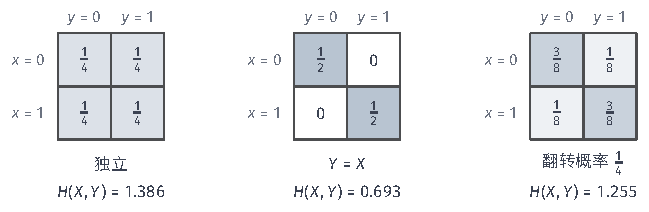
\includegraphics[width=109.8mm]{figures/07-probability/04-distribution-analysis/tikz/info-same-marginals/figure.pdf}
  \caption{三张边缘都是$(\tfrac12,\tfrac12)$的联合概率表，格中数值为$p_{X,Y}(x,y)$，底色越深质量越大。联合熵（nat）随依赖关系改变：独立时最大，$Y=X$时最小，以概率$\tfrac14$翻转时居中。}
  \label{fig:info-same-marginals}
\end{BookInlineFigure}

三张表的共同点是$H(X,Y)\leq H(X)+H(Y)$，独立时取等号；这个不等式在第~\ref{sec:info-mi-entropy}节证明。它说明依赖关系只会让整体更容易确定：一部分不确定性被两个变量“共享”了，不必重复计算。

联合微分熵的例子是二元正态分布。若$\bm{X}\sim\mathcal{N}(\bm{\mu},\bm{\Sigma})$是$d$维正态向量，协方差矩阵$\bm{\Sigma}$正定，对数密度为
\[
  \ln f(\bm{x})=-\frac12\ln\bigl((2\pi)^{d}\det\bm{\Sigma}\bigr)-\frac12(\bm{x}-\bm{\mu})^{\top}\bm{\Sigma}^{-1}(\bm{x}-\bm{\mu}).
\]
二次型的期望是$\operatorname{tr}(\bm{\Sigma}^{-1}\bm{\Sigma})=d$，所以
\begin{equation}
  h(\bm{X})=\frac12\ln\bigl((2\pi\mathrm{e})^{d}\det\bm{\Sigma}\bigr).
  \label{eq:info-gaussian-vector-entropy}
\end{equation}
二维标准化、相关系数为$\rho$时$\det\bm{\Sigma}=1-\rho^{2}$，相关越强，联合微分熵越小，$\lvert\rho\rvert\to1$时趋于$-\infty$。质量越来越集中到一条直线附近，平面上的密度越来越高。

\subsection{条件熵}
\label{sec:info-conditional-entropy}

已知$Y=y$以后，$X$的概率表变成条件分布$p_{X\mid Y}(\cdot\mid y)$：条件化就是只保留$Y=y$的那一列，再重新归一。这张新表的熵，是看到$Y=y$以后$X$剩下的不确定性。不同的$y$留下的不确定性不同，再按$y$出现的概率平均。

\begin{definition}[条件熵]
\label{def:info-conditional-entropy}
设$X,Y$是离散随机变量。对$p_Y(y)>0$的$y$，令
\begin{equation}
  H(X\mid Y=y)=-\sum_xp_{X\mid Y}(x\mid y)\ln p_{X\mid Y}(x\mid y).
  \label{eq:info-conditional-entropy-value}
\end{equation}
$X$在给定$Y$时的\term{条件熵}（conditional entropy）是
\begin{equation}
  H(X\mid Y)=\sum_{y}p_Y(y)\,H(X\mid Y=y)=\mathbb{E}\bigl[-\ln p_{X\mid Y}(X\mid Y)\bigr].
  \label{eq:info-conditional-entropy}
\end{equation}
\end{definition}

式~\eqref{eq:info-conditional-entropy}中第一个和是对式~\eqref{eq:info-conditional-entropy-value}的平均。第二个等号把双重求和合并：$p_Y(y)p_{X\mid Y}(x\mid y)=p_{X,Y}(x,y)$，所以
\[
  H(X\mid Y)=-\sum_{x,y}p_{X,Y}(x,y)\ln p_{X\mid Y}(x\mid y),
\]
各项非负，求和次序可以交换。条件熵是平均剩余不确定性，不是对某一个观测值的保证。

\paragraph{一张不对称的表}
下面这张表在后面几节反复使用：
\begin{equation}
  p_{X,Y}(0,0)=\tfrac14,\quad p_{X,Y}(0,1)=0,\quad p_{X,Y}(1,0)=\tfrac38,\quad p_{X,Y}(1,1)=\tfrac38.
  \label{eq:info-z-table}
\end{equation}
可以把它想成：$X=0$时$Y$必为$0$；$X=1$时$Y$是一枚公平硬币。边缘分布为
\[
  p_X=(\tfrac14,\tfrac34),\qquad p_Y=(\tfrac58,\tfrac38).
\]

按行看，$X=0$那一行条件分布是$(1,0)$，熵为$0$；$X=1$那一行是$(\tfrac12,\tfrac12)$，熵为$\ln2$。按$p_X$平均，
\[
  H(Y\mid X)=\tfrac14\cdot0+\tfrac34\ln2\approx0.520\ \mathrm{nat}.
\]

按列看，$Y=0$那一列的条件分布是$(\tfrac14,\tfrac38)/\tfrac58=(\tfrac25,\tfrac35)$，熵为$h_{\mathrm{b}}(\tfrac25)\approx0.673$；$Y=1$那一列是$(0,1)$，熵为$0$。按$p_Y$平均，
\[
  H(X\mid Y)=\tfrac58\cdot0.673+\tfrac38\cdot0\approx0.421\ \mathrm{nat}.
\]
两个条件熵不相等：条件熵与“谁给定谁”有关。

\begin{BookInlineFigure}
  \centering
  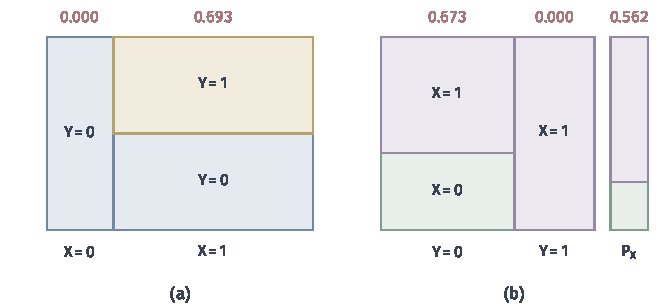
\includegraphics[width=112mm]{figures/07-probability/04-distribution-analysis/matplotlib/info-conditional-slices/figure.pdf}
  \caption{表~\eqref{eq:info-z-table}的条件分布。(a)按$X$分割，宽度为$p_X(x)$，高度为$Y$的条件概率，红色数字为各行的条件熵$H(Y\mid X=x)$。(b)按$Y$分割，宽度正比于$p_Y(y)$，高度为$X$的条件概率，红色数字为$H(X\mid Y=y)$；最右的窄条是无条件的$p_X$及其熵$H(X)\approx0.562$。单位为nat。}
  \label{fig:info-conditional-slices}
\end{BookInlineFigure}

图~\ref{fig:info-conditional-slices}(b)还显示了一个容易误解的现象：$H(X\mid Y=0)\approx0.673$大于$H(X)\approx0.562$。观测到$Y=0$以后，$X$反而更不确定了，因为$Y=0$把原来偏向$X=1$的质量拉向均匀。但这样的观测值只是一部分；$Y=1$时$X$完全确定。平均以后$H(X\mid Y)\approx0.421$，仍小于$H(X)$。第~\ref{sec:info-mi-entropy}节证明这对一切离散变量成立：条件化平均来说不增加熵，但单个观测值可以增加。

\paragraph{离散与连续的区别}
离散时$H(X\mid Y=y)\geq0$，所以$H(X\mid Y)\geq0$，等号当且仅当每个$y$下$X$确定，即$X$是$Y$的函数（除去零概率的$y$）。连续时用条件密度代替条件概率，定义
\[
  h(X\mid Y)=-\iint f_{X,Y}(x,y)\ln f_{X\mid Y}(x\mid y)\,\mathrm{d}x\,\mathrm{d}y,
\]
要求条件密度存在且被积函数绝对可积。它和微分熵一样可以为负，也依赖坐标。

二元标准正态、相关系数$\rho$时，给定$X=x$，$Y$的条件分布是$\mathcal{N}(\rho x,1-\rho^{2})$，与$x$有关的只有均值。每个条件分布的微分熵相同，由式~\eqref{eq:info-gaussian-entropy}，
\begin{equation}
  h(Y\mid X)=\frac12\ln\bigl(2\pi\mathrm{e}(1-\rho^{2})\bigr).
  \label{eq:info-gaussian-conditional-entropy}
\end{equation}
$\rho=0.9$时它约为$0.589$ nat；$\rho^{2}>1-1/(2\pi\mathrm{e})\approx0.941$时它为负数。负值只说明条件密度很窄，不能读成“剩余不确定性为负”。

\subsection{熵的链式法则}
\label{sec:info-entropy-chain-rule}

确定$(X,Y)$可以分两步：先确定$X$，再在已知$X$的情况下确定$Y$。图~\ref{fig:info-chain-tree}把表~\eqref{eq:info-z-table}画成两步的树。第一步的不确定性是$H(X)\approx0.562$；第二步要看走到哪一支，$X=0$那支已无悬念，$X=1$那支还剩$\ln2$，平均$0.520$。两步合起来应当是整体的不确定性。

\begin{BookInlineFigure}
  \centering
  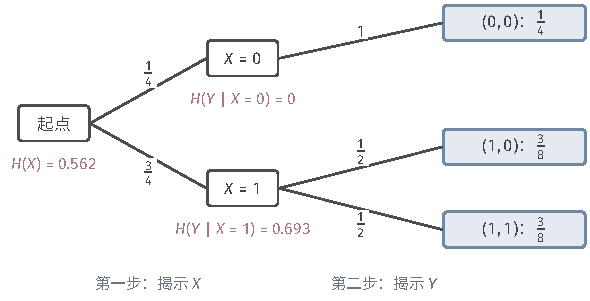
\includegraphics[width=100mm]{figures/07-probability/04-distribution-analysis/tikz/info-chain-tree/figure.pdf}
  \caption{表~\eqref{eq:info-z-table}的两步揭示树。第一步按$p_X=(\tfrac14,\tfrac34)$揭示$X$，第二步按条件分布揭示$Y$；叶子为联合概率。红字为各步的熵（nat），第二步的平均为$\tfrac34\ln2\approx0.520$，与第一步的$0.562$相加得$H(X,Y)\approx1.082$。}
  \label{fig:info-chain-tree}
\end{BookInlineFigure}

\begin{theorem}[熵的链式法则]
\label{thm:info-entropy-chain-rule}
设$X,Y$是离散随机变量，则在$[0,\infty]$中
\begin{equation}
  H(X,Y)=H(X)+H(Y\mid X).
  \label{eq:info-entropy-chain-rule}
\end{equation}
对离散随机变量$X_1,\dots,X_n$，
\begin{equation}
  H(X_1,\dots,X_n)=\sum_{i=1}^{n}H(X_i\mid X_1,\dots,X_{i-1}),
  \label{eq:info-entropy-chain-rule-n}
\end{equation}
其中$i=1$的项理解为$H(X_1)$。
\end{theorem}

\begin{proof}
在$p_{X,Y}(x,y)>0$的点，$p_{X,Y}(x,y)=p_X(x)\,p_{Y\mid X}(y\mid x)$，取负对数，得到
\[
  -\ln p_{X,Y}(x,y)=-\ln p_X(x)-\ln p_{Y\mid X}(y\mid x).
\]
右端两项都非负。乘以$p_{X,Y}(x,y)$后对$(x,y)$求和；非负项的和可以拆开、可以交换次序，即使为$+\infty$也成立。第一项的和是$-\sum_xp_X(x)\ln p_X(x)=H(X)$，第二项的和由式~\eqref{eq:info-conditional-entropy}是$H(Y\mid X)$。

多个变量时，把$(X_1,\dots,X_{n-1})$看成一个变量，对它与$X_n$用式~\eqref{eq:info-entropy-chain-rule}，得到
\[
  H(X_1,\dots,X_n)=H(X_1,\dots,X_{n-1})+H(X_n\mid X_1,\dots,X_{n-1}),
\]
再对前一项归纳即可。
\end{proof}

用表~\eqref{eq:info-z-table}验证。直接计算联合熵，
\[
  H(X,Y)=-\tfrac14\ln\tfrac14-2\cdot\tfrac38\ln\tfrac38\approx1.082.
\]
先揭示$X$，$H(X)+H(Y\mid X)\approx0.562+0.520=1.082$。换一个顺序，$H(Y)=h_{\mathrm{b}}(\tfrac38)\approx0.662$，$H(Y)+H(X\mid Y)\approx0.662+0.421=1.082$，也相同。揭示的顺序不同，每一步分到的不确定性不同，总量不变。

链式法则不要求独立。变量独立时，$p_{X_i\mid X_1,\dots,X_{i-1}}=p_{X_i}$，各条件熵等于无条件熵，式~\eqref{eq:info-entropy-chain-rule-n}化为$\sum_iH(X_i)$。不独立时不能把联合熵写成边缘熵之和，图~\ref{fig:info-same-marginals}已经给出了反例。

\paragraph{移项与连续情形}
链式法则常被移项为$H(Y\mid X)=H(X,Y)-H(X)$。这只在$H(X)<\infty$时有意义；否则右端可能是$\infty-\infty$。例如取$H(X)=\infty$的可数变量并令$Y=X$，$H(X,Y)=\infty$，$H(Y\mid X)=0$，链式法则$\infty=\infty+0$成立，移项却没有意义。

对有联合密度的$(X,Y)$，同样有$f_{X,Y}=f_X\,f_{Y\mid X}$，取负对数后积分，得到
\[
  h(X,Y)=h(X)+h(Y\mid X).
\]
但这里各项可以为负，不能像离散时那样靠“非负项可以拆开”保证等式。需要先核对$f_X\lvert\ln f_X\rvert$与$f_{X,Y}\lvert\ln f_{Y\mid X}\rvert$都可积，这时拆开积分合法，等式成立，并且$h(X,Y)$也有限。二元正态是一个检查的例子：由式~\eqref{eq:info-gaussian-entropy}与式~\eqref{eq:info-gaussian-conditional-entropy}，
\[
  h(X)+h(Y\mid X)=\frac12\ln(2\pi\mathrm{e})+\frac12\ln\bigl(2\pi\mathrm{e}(1-\rho^{2})\bigr),
\]
与式~\eqref{eq:info-gaussian-vector-entropy}在$d=2$、$\det\bm{\Sigma}=1-\rho^{2}$时的值相同。
